% Unofficial University of Cambridge Poster Template
% https://github.com/andiac/gemini-cam
% a fork of https://github.com/anishathalye/gemini
% also refer to https://github.com/k4rtik/uchicago-poster

\documentclass[final]{beamer}

% ====================
% Packages
% ====================

\usepackage[T1]{fontenc}
\usepackage{lmodern}
\usepackage[size=custom,width=120,height=90,scale=1.0]{beamerposter}
\usetheme{gemini}
\usecolortheme{maa}
\usepackage{graphicx}
\usepackage{booktabs}
\usepackage[numbers]{natbib}
\usepackage{tikz}
\usepackage{pgfplots}
\pgfplotsset{compat=1.14}
\usepackage{anyfontsize}
\linespread{1.1}


% ====================
% Lengths
% ====================

% If you have N columns, choose \sepwidth and \colwidth such that
% (N+1)*\sepwidth + N*\colwidth = \paperwidth
\newlength{\sepwidth}
\newlength{\colwidth}
\setlength{\sepwidth}{0.025\paperwidth}
\setlength{\colwidth}{0.3\paperwidth}

\newcommand{\separatorcolumn}{\begin{column}{\sepwidth}\end{column}}

% ====================
% Title
% ====================

\title{Analyzing an organism’s sensors using Maximum Entropy
models with \\ bias, variance, and confusion matrices}

\author{Christopher Wang \inst{1} \and Elianna Schimke \inst{1} \and Tristan Kako \inst{2,3} \and Aiden Gao \inst{3} \and Martina Lamberti \inst{4,5} \and Joost le Feber \inst{5} \and Sarah Marzen \inst{1,6,7}}

\institute[shortinst]{\inst{1} Department of Natural Sciences, Scripps and Pitzer College \samelineand \inst{2} Tufts University, MA \samelineand \inst{3} Pioneer Academics, PA \samelineand \inst{4} Center for Research in Neuroscience of LYON, Bron, France \and \inst{5} University of Twente, The Netherlands \samelineand \inst{6} Claremont McKenna College \samelineand \inst{7} National Institute for Theory and Mathematics in Biology, IL}

% ====================
% Footer (optional)
% ====================

\footercontent{
  MAA Socal-Nevada Section Meeting 2026, USC --- MAR-2026 \hfill
  \href{mailto:smarzen@natsci.claremont.edu}{smarzen@natsci.claremont.edu}}
% (can be left out to remove footer)

% ====================
% Logo (optional)
% ====================

% use this to include logos on the left and/or right side of the header:
% \logoright{\includegraphics[height=7cm]{logo1.pdf}}
% \logoleft{\includegraphics[height=7cm]{logo2.pdf}}

% ====================
% Body
% ====================

\begin{document}

% Refer to https://github.com/k4rtik/uchicago-poster
% logo: https://www.cam.ac.uk/brand-resources/about-the-logo/logo-downloads
\addtobeamertemplate{headline}{}
{
    \begin{tikzpicture}[remember picture,overlay]
      \node [anchor=north west, inner sep=3cm] at ([xshift=0.0cm,yshift=1.0cm]current page.north west)
      {
\includegraphics[height=7cm]{logos/kecksci.jpeg}}; 
    \end{tikzpicture}
}

\begin{frame}[t]
\begin{columns}[t]
\separatorcolumn

\begin{column}{\colwidth}

  \begin{block}{Introduction}

    All living organisms use external stimuli to navigate their environment via their sensors. Because encoding information costs energy, organisms retain only a fraction of the information received from their sensors, ideally information that maximizes their ability to remember past environmental states or predict future ones, key functions that support survival. To better understand how well sensor systems absorb stimulus information, we used stimulus-dependent Maximum Entropy (MaxEnt) models with maximum likelihood estimation and typical statistical metrics, such as confusion matrices or bias and variance. In this poster, we apply MaxEnt to investigate cooperativity (using bias and variance) and memory/prediction in neural systems (using confusion matrices). This approach provides two primary benefits over previous approaches: it is more computationally efficient, and it provides a more information-rich picture on how sensors interact with stimulus.

  \end{block}

  \begin{block}{Materials and Methods}

Statistical mechanical models serve as stimulus-dependent Maximum Entropy (MaxEnt) models, yielding $p_\mathrm{model}(s\mid x)$, where $s$ is the sensor state and $x$ is the environmental variable. Here we use Bayes' theorem,
\begin{equation}
    p(x\mid \mathbf{s}) = p(\mathbf{s}\mid x)p(x) / p(\mathbf{s}),
\end{equation} 
and assuming a uniform prior $p(x)$, we form a Maximum Likelihood Estimator (MLE) $\hat{x}(\mathbf{s}) = \arg\max_x p_\mathrm{model}(\mathbf{s}\mid x)$. 

\heading{Estimator Construction for Ordered Variables}
With the MLE in hand, we evaluate the estimator's quality as a function of the true environmental state via
\begin{eqnarray}
\mathrm{Bias}(x) &=& \langle \hat{x}(s)\rangle_{p_\mathrm{model}(s|x)} -x \\
\mathrm{Var}(x) &=& \langle (\hat{x}(s)-\langle\hat{x}(s)\rangle_{p_\mathrm{model}(s|x)})^2 \rangle_{p_\mathrm{model}(s|x)} \\
\mathrm{MSE}(x) &=& \langle \left(\hat{x}(s)-x\right)^2\rangle_{p_\mathrm{model}(s|x)}.
\end{eqnarray}
To investigate cooperativity—a case where we draw new insights using MaxEnt—we use a two-site Adair model in which two binding sites $s_1, s_2$ interact with ligand concentration $x$ through a partition function
\begin{equation}
    Z = 1 + 2 (x/k) + e^{-\beta\Delta\epsilon}(x/k)^2,
\end{equation}
where $K$ is the dissociation constant and $\beta\Delta\epsilon$ is a cooperativity parameter: negative values correspond to positive cooperativity (binding at one site favors binding at the other) and positive values to negative cooperativity.

\heading{Neural system experimental setup}

\begin{columns}

\begin{column}{0.45\linewidth}
    \begin{figure}
        \centering
        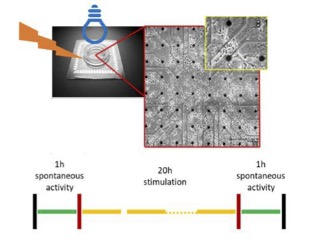
\includegraphics[width=\linewidth]{figs/lamberti23ex.jpg}
        \caption{Example of MEA with cultured neuronal networks and stimulation
protocol.}
        \label{fig:MEA}
    \end{figure}
    \end{column}
    \hfill
    \begin{column}{0.45\linewidth}
        
        Newborn rat neurons were placed on multi-electrode arrays (MEAs) and incubated for 3 weeks in the following conditions: $36^\circ $C, high humidity, and 5\% $\text{CO}_2$. 59 electrodes were connected to the system to measure activity at a sampling frequency of 16 kHz. We recorded 20 hours of light (global) or electrical (focal) stimulation with 1 hour of spontaneous activity on either side. Focal electrical stimulation was applied through one single electrode and global (optogenetic) stimulation used LED pulses placed above the MEA.
    \end{column}
\end{columns}

\vspace{2em}

\heading{Data Processing and Model Fitting for the Neural System}
Our estimator guesses stimulus in/activity (categorical variable), so it is most productive to characterize model performance by generating confusion matrices against the true stimulus. The confusion matrix tells us how often we correctly guess stimulus activity (true positive rate, TPR), stimulus inactivity (true negative rate, TNR), and how often we mistake one for the other. From this, we can derive a predictive accuracy, indicating how often our model makes a correct guess.
\end{block}
\end{column}

\separatorcolumn

\begin{column}{\colwidth}
\begin{block}{Materials and Methods (continued)}
Neural activity and stimulus were binned into successive windows of width $\Delta t = 100$ ms, where one or more spikes in a window yields a 1 and no spikes yields a 0, producing a binary matrix. We fit a joint MaxEnt spin-glass Ising model to estimate the coupling matrix $J$ via
\begin{equation}
    p_\mathrm{model}(x,\mathbf{s}) \propto \exp\bigg( -
    \begin{pmatrix}
        x & \mathbf{s}
    \end{pmatrix}
    \underbrace{
    \begin{pmatrix}
        J_{xx} & J_{xs} \\ J_{sx} & J_{ss}
    \end{pmatrix}
    }_{J}
    \begin{pmatrix}
        x \\ \mathbf{s}
    \end{pmatrix}\bigg),
\end{equation}
whose leading entry $J_{xx}$ captures the firing propensity of the stimulus, off-diagonal blocks $J_{xs}$ and $J_{sx}$ encode stimulus–network correlations, and whose diagonal block $J_{ss}$ captures network–network interactions. The stimulus channel was time-shifted relative to network activity by up to $\pm 200$ ms to probe memory (negative shifts) and prediction (positive shifts). The fitted $J$ matrix was then used to compute the likelihood ratio
\begin{equation}
    L(s) = \frac{p(x=1 \mid s)}{p(x=0 \mid s)} = \exp\left(J_{xx}+J_{xs}s+s^{\top}J_{sx}\right).
\end{equation}
If $L(s) > 1, \hat{x}(s)=1$, otherwise $\hat{x}(s)=0$.
\end{block}

  \begin{block}{Results and Discussion}
  \heading{Cooperativity in Sensors}
Fig \ref{fig:bias} shows bias, variance, and MSE for the two-site Adair model across a range of cooperativities $\beta\Delta\epsilon$. Cooperativity reshapes which ligand concentrations the sensor estimates well: there exists a range of concentrations for which positive cooperativity lowers MSE relative to the independent case ($\beta\Delta\epsilon = 0$), and a complementary range for which it does not. This stands in contrast to a standard mutual information (MI) analysis, which finds that conditionally independent sensors always transmit more total information. Our analysis reveals that the answer to whether cooperativity benefits sensing depends on which ligand concentrations the organism is likely to encounter, a nuance invisible to MI alone.
\begin{figure}
    \centering
    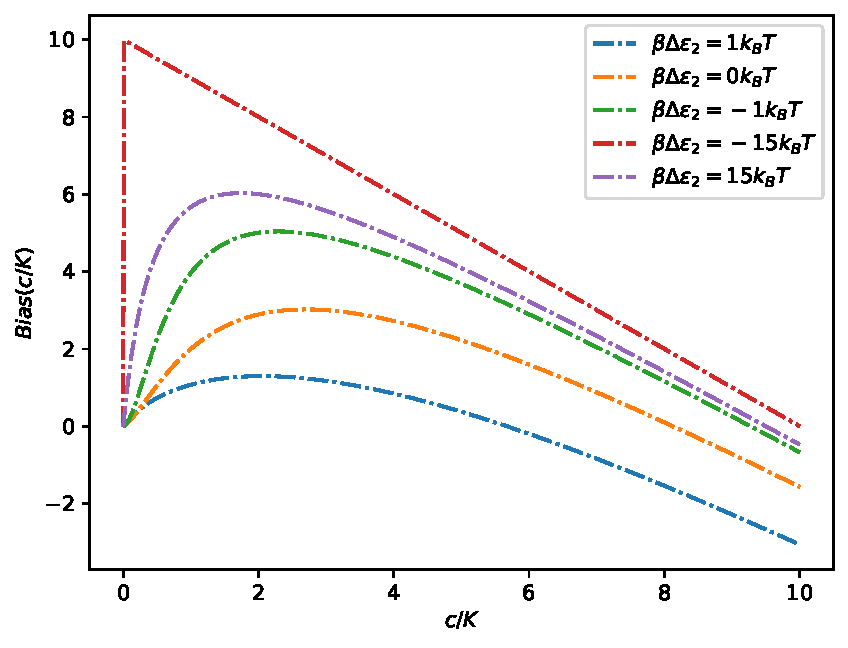
\includegraphics[width=0.3\linewidth]{figs/figurebiaslegend5.pdf}
    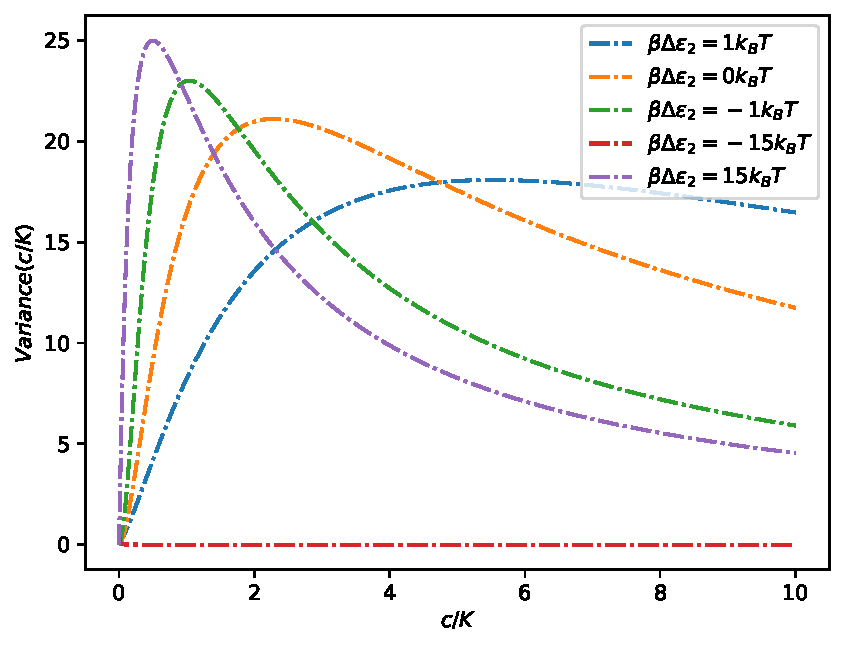
\includegraphics[width=0.3\linewidth]{figs/figurevariancelegend5.pdf}
    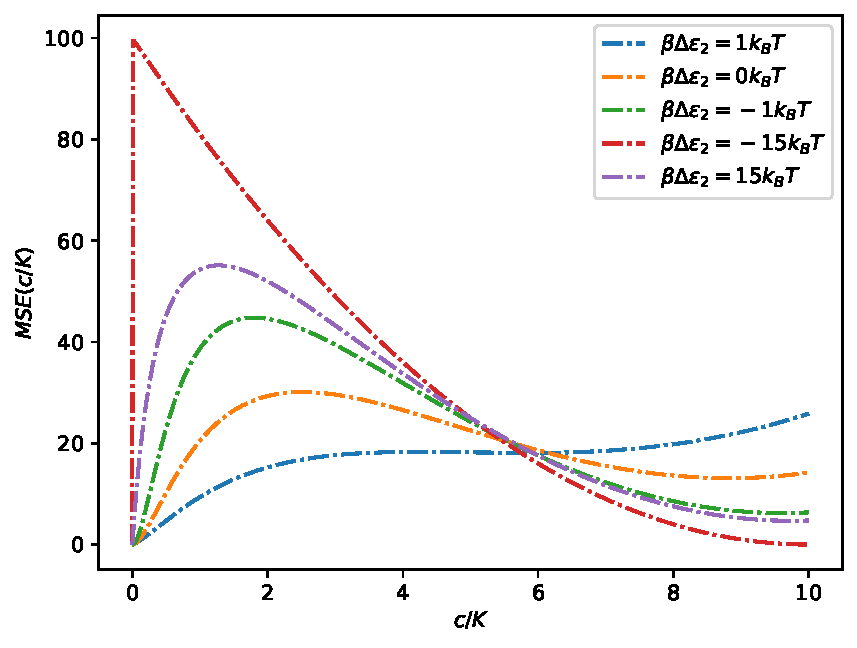
\includegraphics[width=0.3\linewidth]{figs/figuremselegend5.pdf}
    \caption{The bias, variance, and MSE of a sensor with varying degrees of cooperativity. At left, bias as a function of the chemoattractant concentration $c$. In the middle, variance as a function of the chemoattractant concentration $c$. At right, mean-squared error (MSE) as a function of the chemoattractant concentration $c$. A range of cooperativities based on varying $\beta\Delta \epsilon$ are shown.}
    \label{fig:bias}
\end{figure}
\heading{Memory and Prediction in Cultured Neurons}
\begin{figure}
    \centering
    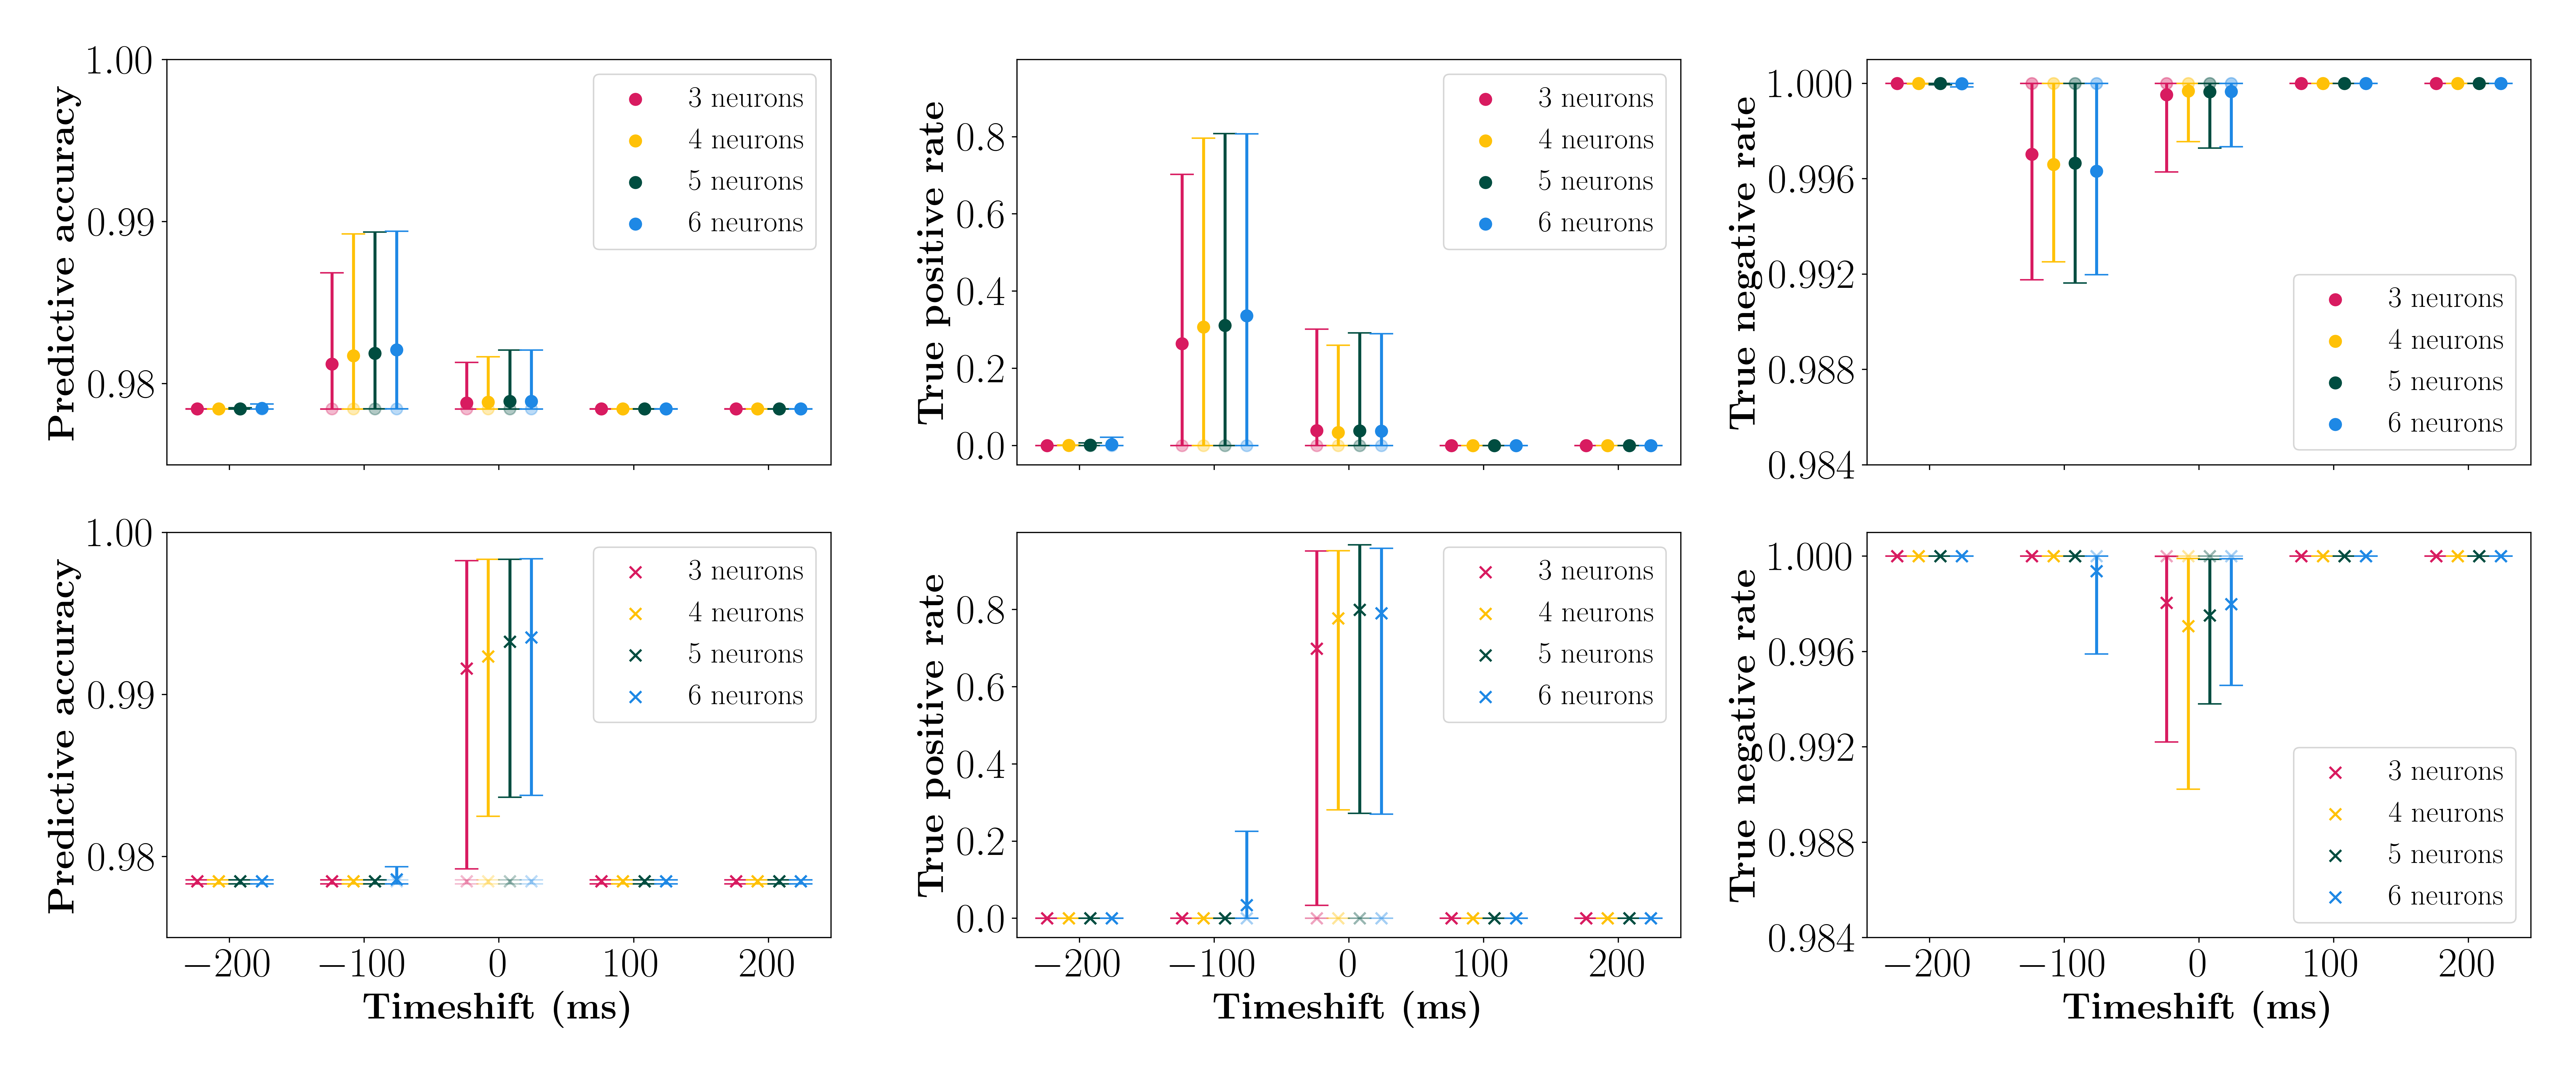
\includegraphics[width=\linewidth]{figs/cm metrics revised.png}
    \caption{Predictive accuracy, true positive rate, and true negative rate for baseline and model estimators with $95\%$ confidence intervals. Circular markers denote optogenetic ($n=10$) stimulation (top row), crossed markers denote electrical ($n=8$) stimulation (bottom row). Plots with varying system sizes at the same time-shift are staggered to enhance visibility of markers and error bars.}
    \label{fig:cm metrics}
\end{figure}
\end{block}
\end{column}

\separatorcolumn

\begin{column}{\colwidth}
\begin{block}{Results and Discussion (continued)}

\begin{figure}
    \centering
    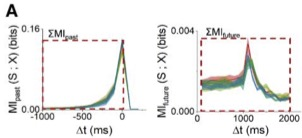
\includegraphics[width=0.7\linewidth]{figs/lamberti23.jpg}
    \caption{An example of $\mathrm{MI}_\mathrm{past}$ and $\mathrm{MI}_\mathrm{future}$. Taken from Fig 3A of \cite{lamberti2023prediction}.}
    \label{fig:MI}
\end{figure}

Fig \ref{fig:cm metrics} shows that electrical stimulation yields the strongest improvement over baseline at 0 ms time-shift (mean predictive accuracy 99.35\%, TPR 79.05\%), while optogenetic stimulation peaks at $-100$ ms (predictive accuracy 98.21\%, TPR 33.64\%). Even selecting just the three most informative electrodes captures the majority of possible improvement, with diminishing returns at larger subsystem sizes. Notably, no system displayed predictive behavior: at time-shifts of $+100$ ms and beyond, all metrics returned to baseline. This is consistent with MI analyses, which found $\mathrm{MI}_\mathrm{future} \sim 10^{-3}$ bits (mutual information of prediction) compared to $\mathrm{MI}_\mathrm{past} \sim 10^{-1}$ bits (mutual information of memory). The predictive signal is likely too weak to cross the likelihood ratio threshold, while the memory signal is strong enough to drive improvements. Moreover, confusion matrices add granularity: it separately quantifies how often the network mistakes silence for activity versus the reverse.

We also experimented with changing time bin size and decomposing each experiment into hourly chunks, but found no statistically significant trends.

\end{block}

  \begin{alertblock}{Conclusion}
We combined stimulus-dependent and joint MaxEnt models with maximum likelihood estimation to analyze biosensors using bias, variance, and confusion matrices, metrics that provide a richer picture than MI alone. For ordinal variables, bias and variance as functions of ligand concentration revealed that cooperativity can improve estimation at specific concentration ranges, a trend invisible to MI. For categorical variables, confusion matrices quantified memory and prediction in cultured neurons, showing strong memory signatures consistent with prior MI analyses while additionally resolving error types across activity and inactivity.
  \end{alertblock}

  \begin{block}{References}

    \nocite{*}
    \footnotesize{\bibliographystyle{plainnat}\bibliography{poster}}

  \end{block}

    \begin{block}{Acknowledgements}

    \footnotesize{This work was performed in part at the Aspen Center for Physics and was supported by a grant from the Alfred P. Sloan Foundation (G-2024-22395). This study was supported by the US Air Force Office for Scientific Research, Grant Number FA9550-19-1-0411. Research was sponsored by the Army Research Office and was accomplished under Grant Number W911NF-25-1-0260.}

  \end{block}

\end{column}

\separatorcolumn
\end{columns}
\end{frame}

\end{document}
